% Euclidean Handout Number nine
\documentclass{tufte-handout}

%\geometry{showframe}% for debugging purposes -- displays the margins

%%%% Packages to make things pretty
\usepackage{amsmath,amsthm}
\usepackage{booktabs}
\usepackage{graphicx}
\setkeys{Gin}{width=\linewidth,totalheight=\textheight,keepaspectratio}
\graphicspath{{graphics/}}
\usepackage{units}
\usepackage{fancyvrb}
\fvset{fontsize=\normalsize}
\usepackage{multicol}
\usepackage{pdfpages}

%%%% Theorem Environments
\theoremstyle{definition}
\swapnumbers
\newtheorem{problem}{Problem}[section]
\newtheorem{conjecture}[problem]{Conjecture}
\newtheorem*{definition}{Definition}
\newtheorem*{theorem}{Theorem}
\newtheorem{question}[problem]{Question}
\newtheorem{challenge}[problem]{Challenge}
\newtheorem*{postulate}{Postulate}

%%%%%

\title{Euclidean Geometry:\\An Introduction to Mathematical Work}
\author[]{Math 3600}
\date{Spring 2018}

\begin{document}

\maketitle

\begin{marginfigure}
    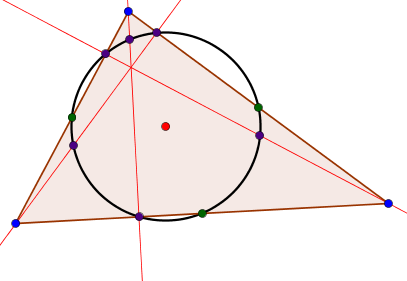
\includegraphics{NPC}
\end{marginfigure}

\setcounter{section}{9}
\section{Circles}

We have learned quite a bit about basic polygonal shapes, especially triangles, and various species of quadrilaterals. Now we turn our attention to circles. This is the subject of Book III in Euclid's \emph{Elements}. We already have one beautiful theorem about circles, that of Thales, but we'd like to have more.

\marginnote[15pt]{Pay special attention to III.16, III.18, III.20, III.21, III.31 and III.32.}

Read the \emph{Elements} Book III Propositions 1-34. For the following propositions you should work in the axiomatic style of Euclid using I.1-34,  III.1-34 and any previously proved results.



\begin{conjecture}\label{conj:tangents-to-circle}
Let $AB$ and $AC$ be two tangent lines from a point $A$ outside a circle. Then $AB$ is congruent to $AC$.
\end{conjecture}

\begin{definition}\label{defn:circles-perp}
We say that two circles \emph{meet at right angles} if the radii of the two circles to a point of intersection make a right angle.
\end{definition}

\begin{conjecture}\label{conj:perp-circles}
Let $\Gamma$ and $\Omega$ be two circles with centers $G$ and $O$, respectively. Suppose that these circles meet at two points $A$ and $B$. If $GAO$ is a right angle, then $GBO$ is a right angle.
\end{conjecture}


\begin{definition}\label{defn:cyclic-quad}
A quadrilateral $ABCD$ is said to be a \emph{cyclic quadrilateral} if there is a circle $\Gamma$ such that the four vertices $A,B,C$ and $D$ lie on $\Gamma$.
\end{definition}

\begin{conjecture}\label{conj:rect-cyclic}
A rectangle is always a cyclic quadrilateral.
\end{conjecture}

\begin{conjecture}[Cyclic Quadrilateral Theorem]\label{conj:angles-cyclic-quad}
Let $A,B,C$ and $D$ be four points. The quadrilateral $ABCD$ is cyclic if and only if angle $DAC$ is congruent to $DBC$.
\end{conjecture}


\begin{conjecture}\label{conj:tangent-to-two-circles}
Let two circles be tangent at a point $A$. If two lines are drawn through $A$ meeting one circle at further points $B$ and $C$ and meeting the other circle at points $D$ and $E$, then $BC$ is parallel to $DE$.
\end{conjecture}


\vfill
\end{document}

%sagemathcloud={"zoom_width":100}